
%(BEGIN_QUESTION)
% Copyright 2012, Tony R. Kuphaldt, released under the Creative Commons Attribution License (v 1.0)
% This means you may do almost anything with this work of mine, so long as you give me proper credit

Sketch the graphical interpretation of the derivative $dy \over dx$ at the point specified on the graph (the red dot), and determine whether its value is {\it positive} or {\it negative}:

$$\includegraphics[width=15.5cm]{i01347x01.eps}$$

\underbar{file i01347}
%(END_QUESTION)





%(BEGIN_ANSWER)

$$\includegraphics[width=15.5cm]{i01347x02.eps}$$

$dy \over dx$ has a {\it negative} value at the red dot because the differential $dy$ is negative while the differential $dx$ is positive.

%(END_ANSWER)





%(BEGIN_NOTES)


%INDEX% Mathematics, calculus: derivative (defined in a graphical sense)

%(END_NOTES)


